
In this section, we analyze $9,600$ simulated communities\footnote{$4$ models, $(40+20)$ objective and subjective questions, $10$ random graphs and lattices, and $4$ independent episodes for each group trajectory in each configuration. We use the word episodes to refer to the independent random samples with the same configuration. Together with the out-of-distribution generalization and asynchronous-update experiments, the full dataset comprises over $10{,}000$ groups, which is the figure quoted in the abstract.} to empirically characterize the individual- and group-level dynamics of the agents. Throughout this section, we conduct our analysis using the continuous values of opinions, $\bar{o}_i(t) \in [ -1, +1]$.

\subsection{Behavior of Groups and Individuals }\label{sec:macrostates_microstates}


\begin{figure}[!ht]
    \centering    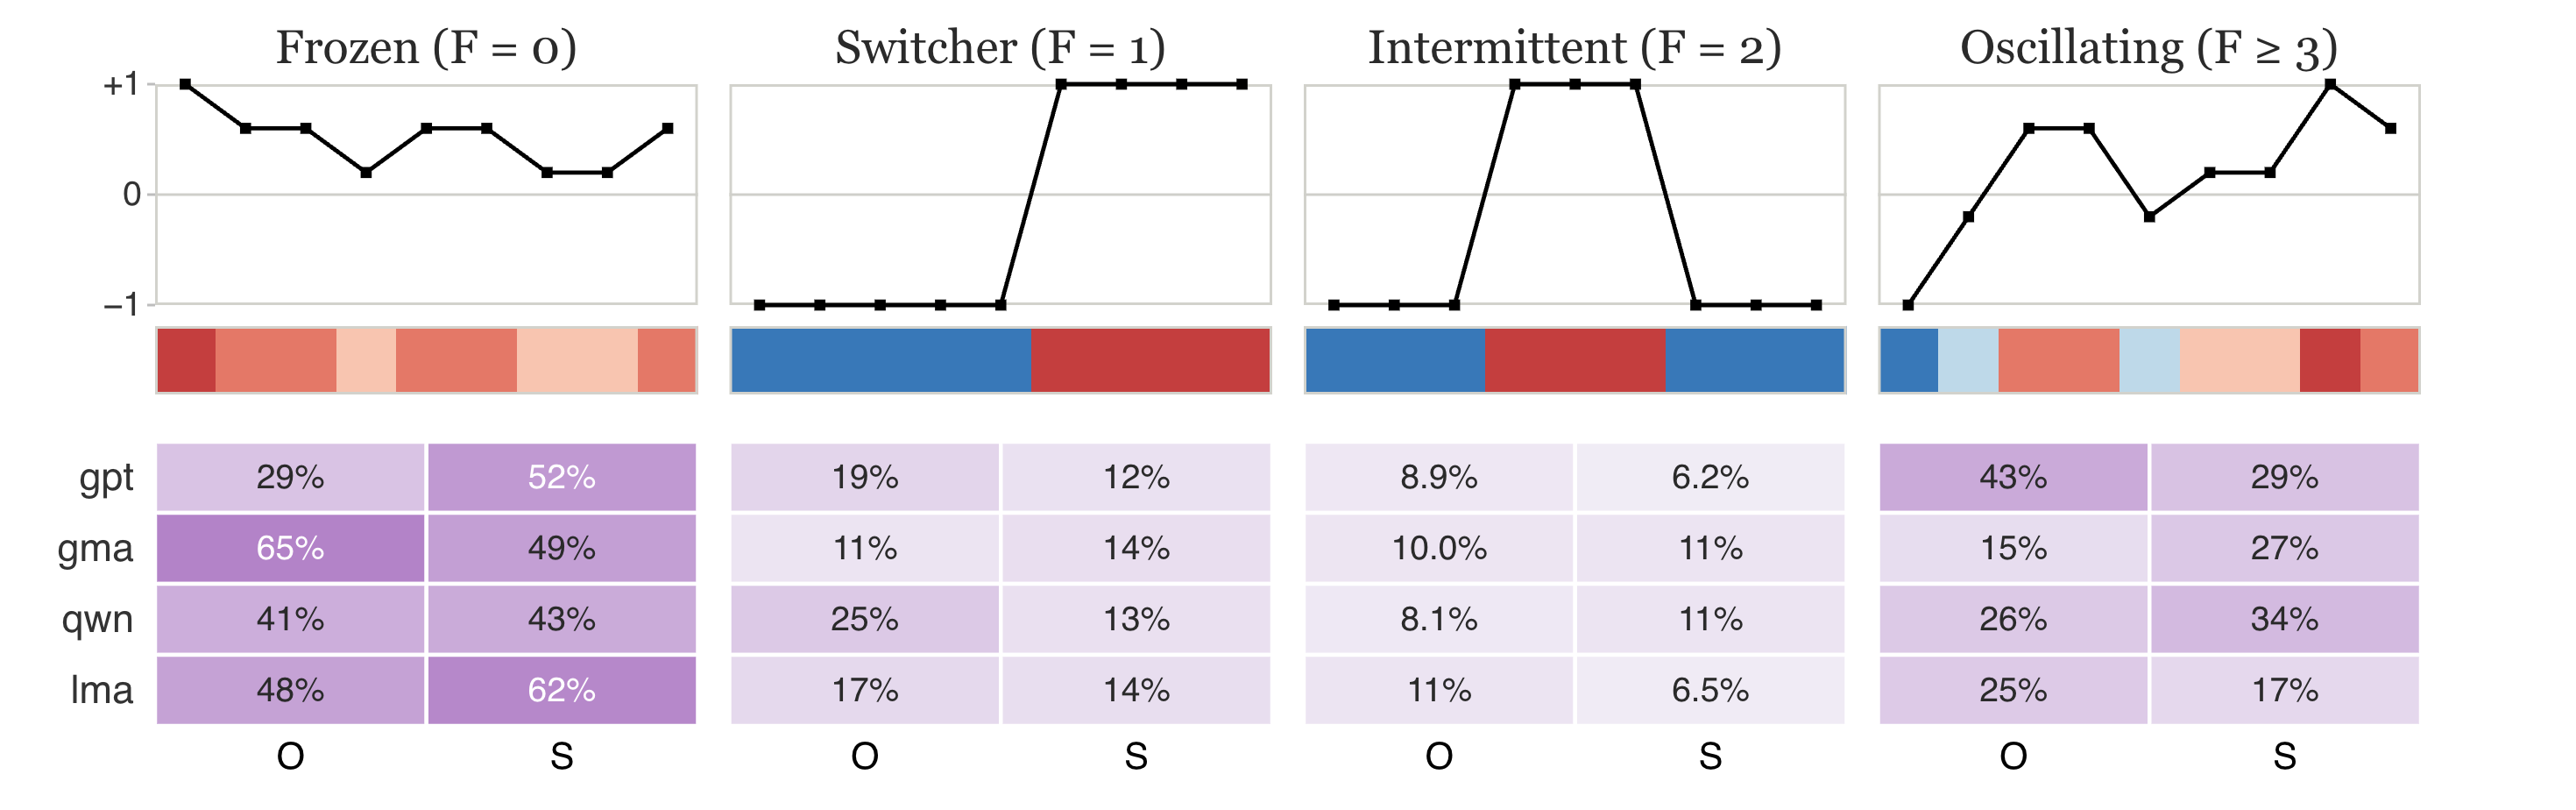
\includegraphics[width=0.9\textwidth]{main/Figures/main_02_agent_microstates.png}
    \caption{\textit{Individual Archetypes. Individual trajectories are classified into four distinct archetypes, with the prevalence of archetypes varying across models and between objective and subjective questions.} The line plot and the heatmap show individual trajectories $
(\bar{o}_i(0),  \bar{o}_i(1), \dots, \bar{o}_i(T))
$. The table below shows the distribution of individual archetypes across different models (GPT-4o-mini (gpt), Gemma-3n-E4B-it (gma), Qwen3.5-9B (qwn), and Llama-3.1-8B-Instruct (lma)) for the objective (O) and subjective (S) questions.}
\label{fig:microstates}
\end{figure}
\begin{figure}[!ht]
    \centering
    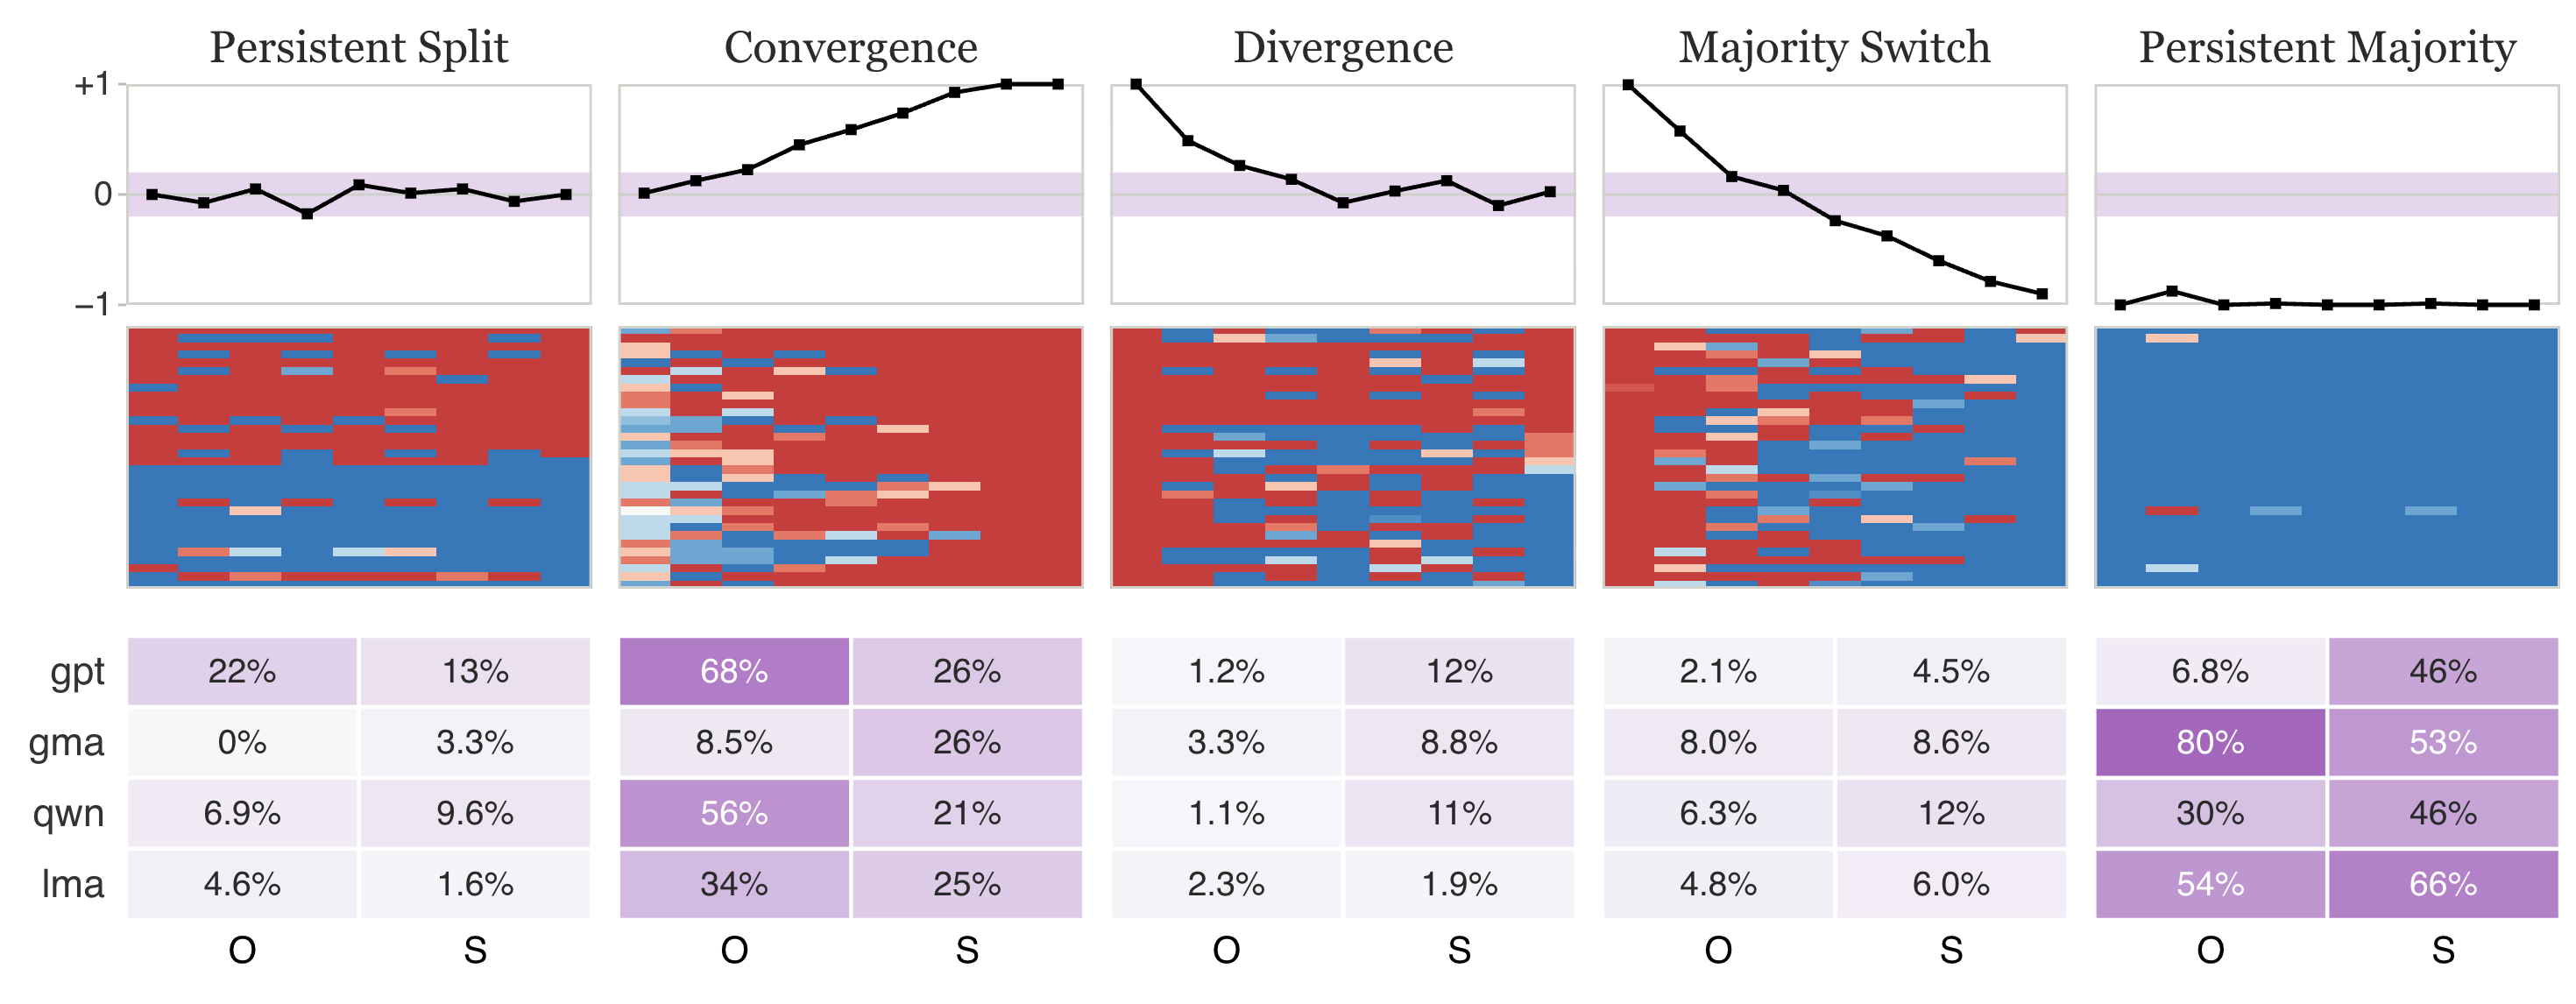
\includegraphics[width=0.99\textwidth]{main/Figures/main_03_society_macrostates.png}
\caption{\textit{Group Archetypes. Group trajectories exhibit five distinct archetypes whose prevalence varies substantially across models and question types. While some groups uninterestingly lock into a persistent majority, many others converge, diverge, switch majorities, or remain  as a persistently split.} The heatmap and line plot demonstrate an example group trajectory belonging to each of the five group archetypes. Row $i$ of the heatmap shows the individual trajectory, $ (\bar{o}_i(0),  \bar{o}_i(1), \dots, \bar{o}_i(T))
$, of $i$th agent in the group. Column $j$ of the heatmap is a snapshot of the individual opinions at timestep $j$: $ (\bar{o}_1(j),  \bar{o}_2(j), \dots, \bar{o}_N(j))
$. The line plot shows the trend in net opinion \(
n(t)
\) across timesteps. The table below shows the distribution of group archetypes. O and S indicate objective and subjective questions.}\label{fig:macrostates}
\end{figure}

\textit{Individuals.} We denote the opinion of a single agent at a timestep  with $\bar{o}_i(t) \in [ -1, +1]$. An individual trajectory is the sequence of one agent's opinions over time: 
$
(\bar{o}_i(0),  \bar{o}_i(1), \dots, \bar{o}_i(T))
$. By tracing individual trajectories across time, we assign each individual to one of four mutually exclusive and exhaustive archetypes based on how many times they switch sides, \textit{i.e.}, 
\[
F_i=\sum_{t=0}^{T-1}\mathbf{1}\!\left\{\text{sign}(\bar{o}_i(t))\neq \text{sign}(\bar{o}_i(t+1))\right\}=\sum_{t=0}^{T-1}\mathbf{1}\!\left\{s_i(t)\neq s_i(t+1)\right\},\]
where \(\mathbf{1}\{\cdot\}\) is the indicator function. In Figure~\ref{fig:microstates}, we show the (1) \emph{Frozen} agents do not change their opinion throughout the interaction and opinion update rounds ($F_i=0$ switches), (2) \emph{Switchers} start with an opinion and end up with the opposite opinion at the end of the 8 rounds after a single switch ($F_i=1$ switch), (3) \emph{Intermittent} agents are those that switch their opinion and switch it back ($F_i=2$ switches), and (4) \emph{Oscillators} are those that switch their opinion more than twice ($F_i>2$ switches). We observe that the distribution across these archetypes is uneven: frozen agents dominate in most settings followed by oscillators, while switchers and intermittent are comparatively rare.

\textit{Groups.} We refer to the collective opinion trajectory of all $N$ agents as a \textit{group trajectory}, which is an $N \times (T+1)$ matrix whose columns are the successive group opinions and whose rows are the individual trajectories. Running the system on a given $(\{p_i\}_{i=1}^N,\ q,\ J)$ produces one such trajectory, capturing how opinions evolve over time. We also classify group trajectories based on how many times they switch sides. We define a group’s \textit{net opinion} as \(n(t) = \frac{1}{N}\sum_i \bar{o}_i(t)\). Although it is possible to count the number of times \(n(t)\) changes sign, analogous to the classification rule we followed in the individual trajectories, this is not particularly informative for group opinions because minor fluctuations around zero can result in multiple switches that are not meaningful. To address this issue, we define a \textit{split band} \([-\delta, \delta]\) around zero and let
\[
\tilde{n}(t) =
\begin{cases}
+1, & \text{if } n(t) \geq \delta, \\
-1, & \text{if } n(t) \leq -\delta, \\
0,  & \text{otherwise}.
\end{cases}
\]
Using the initial ($\tilde{n}(0)$) and final ($\tilde{n}(T)$) net opinions,\footnote{We use $T=8$ in our experiments as  communities typically converge before 8 iterations.} we classify the group trajectories into $5$ mutually exclusive and exhaustive \textit{group archetypes}.\footnote{Note that the split band is already implicitly defined at the level of individual trajectories. Since
$\bar{o}_i(t)$ is the mean of $K=5$ binary votes in $\{-1,+1\}$, it takes values
only on the grid $\{-1,-0.6,-0.2,+0.2,+0.6,+1\}$, whose smallest nonzero
magnitude is $1/K = 0.2$; and because $K$ is odd, $\bar{o}_i(t)=0$ cannot occur.
The band $(-\delta,\delta)$ with $\delta = 1/K = 0.2$ is therefore already implicitly used
for individual trajectories. We therefore fix the value of $\delta =0.2$, which is the resolution of a single agent's opinion, so
$|n(t)| < 1/K$ means the population average falls below the finest distinction
any individual agent is able to express.} For groups with no clear initial majority (start inside the split band with ($\tilde{n}(0) = 0$), \emph{Persistent Split} ends the 8th round inside the split band ($\tilde{n}(8) = 0$), while \emph{Convergence} ends outside the split band, having converged to a clear majority ($\tilde{n}(8) \neq 0$). For groups with a clear initial majority (start outside the split band with $\tilde{n}(0) \neq 0$), \emph{Persistent Majority} ends the 8th round as the same initial majority opinion ($\tilde{n}(0) \cdot \tilde{n}(8)  > 0$), \emph{Divergence} ends inside the split band ($\tilde{n}(0) \cdot \tilde{n}(8)  = 0$), and \emph{Majority Switch} ends on the opposite side of the split band ($\tilde{n}(0) \cdot \tilde{n}(8)  < 0$).

In Figure \ref{fig:macrostates}, we examine the distribution of different group archetypes and observe that the collective behavior is rich. Notably, \emph{Divergence} and \emph{Majority Switch}, in which the initial majority weakens or is overturned are not rare, reaching $11-12\%$ in GPT-4o-mini and Qwen3.5-9B. Additionally, we also present and discuss $4$ rare non-monotonic group archetypes in Figure \ref{fig:rare_macrostates} and Appendix \ref{apdx:rare_macrostates}. Notably, communication networks can cause consistent differences in group trajectories of the same question (Appendix \ref{apdx:communication_effect}).

\begin{figure}[t]
    \centering
    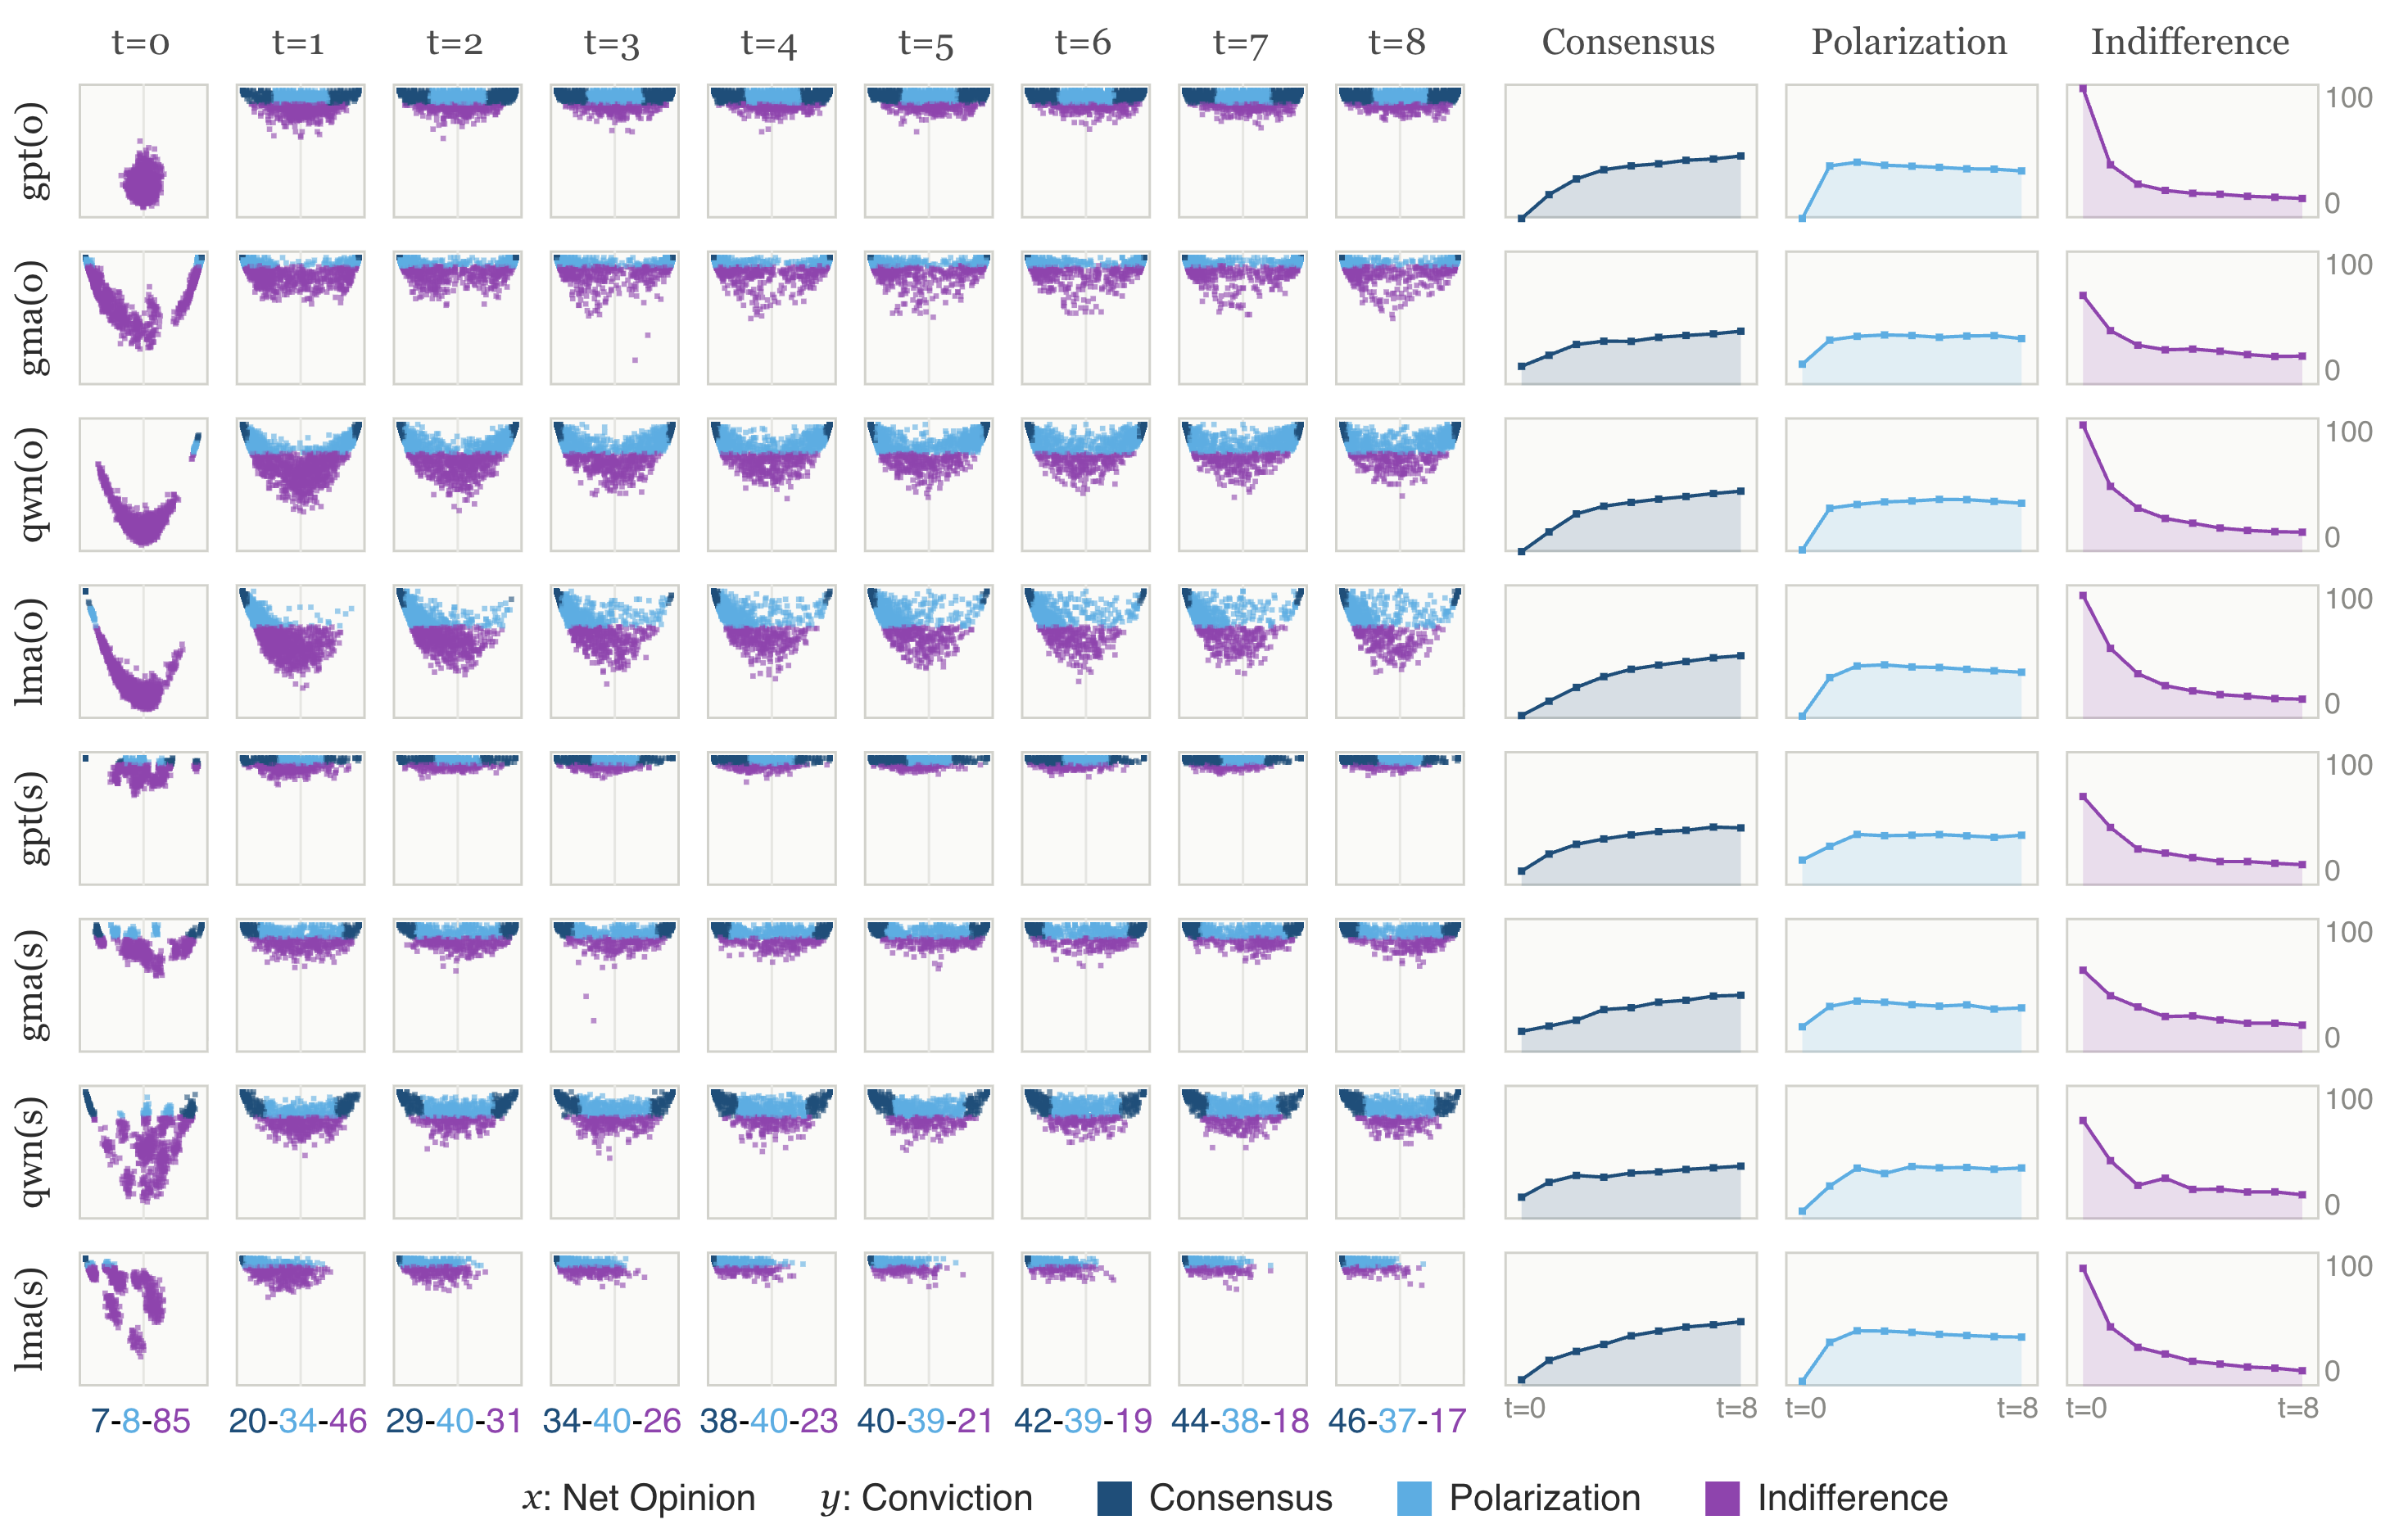
\includegraphics[width=0.99\textwidth]{main/Figures/main_04_macrostate_modes.png}
    \caption{\textit{Conviction Buildup and Consensus Formation.} Each dot represents a group trajectory represented as a point on the net opinion ($x$) and conviction ($y$) plane. By construction, each row is split into approximately equal number of indifference, consensus and polarization examples. The numbers below each column indicate the percentage of examples that fall into each characteristic regimes at that time step, aggregated across all model–regime pairs.}
    \label{fig:3_Observations_modes}
\end{figure}

\begin{figure}[t]
    \centering
    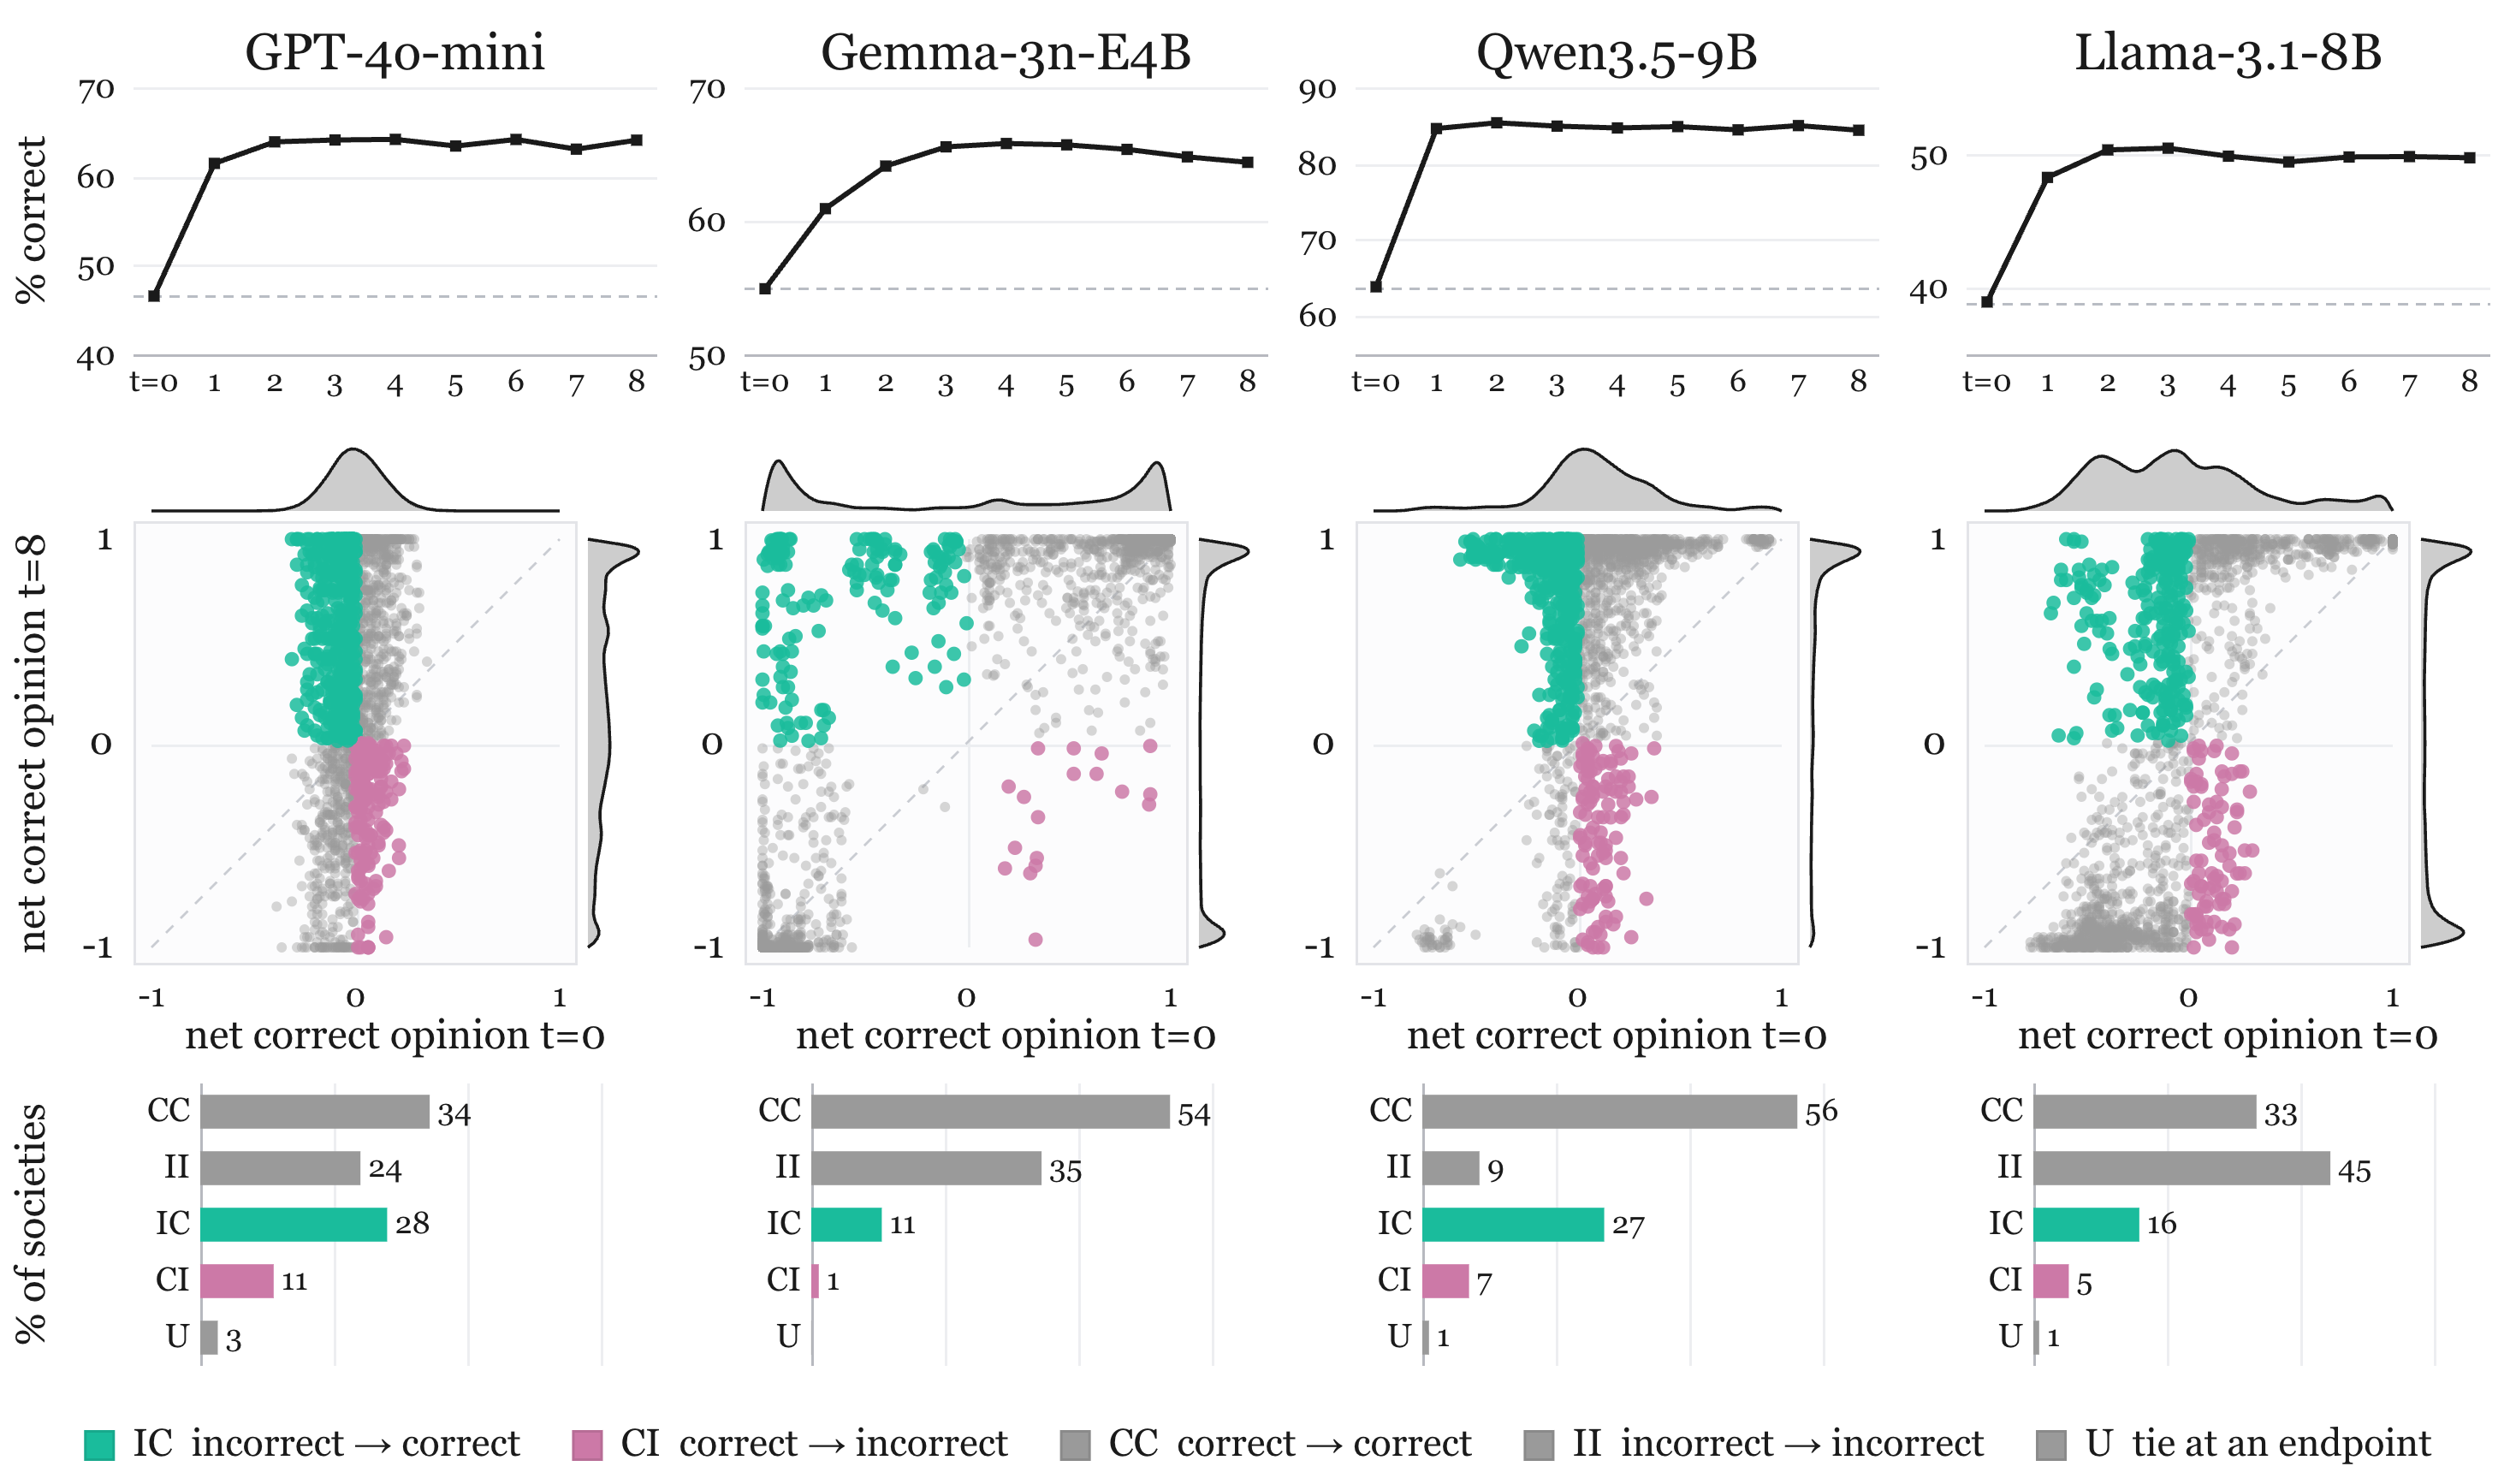
\includegraphics[width=0.99\textwidth]{main/Figures/main_05_truth_seeking.png}
    \caption{\textit{Truth-seeking tendency.} How opinions move toward the correct answer over a run ($6,400$ group trajectories from objective questions only, from signed random graphs and the square and triangular lattices). In a group trajectory, an opinion is represented as true if net opinion has the correct sign. \emph{Row 1:} $y$-axis: percentage of group trajectories, where the net opinion $n(t)$ has the correct sign at round $t$. $x$-axis: timesteps. \emph{Row 2:} Each point represents a group trajectory, which is plotted based on its initial ($t=0$, $x$-axis) and final ($t=8$, $y$-axis) net opinion $n(t)$ multiplied by the sign of the correct answer of the questions to get \textit{net correct opinion}: $n(t) \cdot y_{gt}$, where $y_{gt} \in \{-1, +1\}$ denotes the ground truth answer to the objective question. \emph{Row 3:} Groups switch between being correct and incorrect at $t=0$ and $t=8$. CC (correct$\to$correct), CI (correct$\to$incorrect), IC (incorrect$\to$correct), II (incorrect$\to$incorrect), and U (undecided, $50\text{-}50$ tie at $t=0$ or $t=8$). The two transition categories CI and IC are highlighted.}
\label{fig:3_Observations_ts}
\end{figure}


\subsection{Conviction Buildup and Consensus Formation}
\label{sec:obs_phase_char}

When the net opinion, \(
n(t) = \frac{1}{N}\sum_i \bar{o}_i(t)
\), is close to $+1$ or $-1$, the collective opinion is straightforward to interpret as it means most individuals hold strong opinions that are aligned in the same direction (\textit{consensus}). In contrast, a net opinion close to zero can arise in two fundamentally different ways. In the first case (\textit{polarization}), individuals hold strong opinions (close to +1 or -1), but they are evenly split between opposing viewpoints.  In the second case (\textit{indifference}), most individuals are uncertain or indifferent about their position, and aggregating these weak preferences naturally yields a collective opinion near zero. To characterize this distinction, we define conviction as a measure of how strongly opinionated agents are at a given timestep \(
c(t) = \frac{1}{N}\sum_i \bar{o}_i^2(t)
\). 

In Figure~\ref{fig:3_Observations_modes}, we follow the joint distribution of net opinion ($x$) and conviction ($y$) for all eight model-regime settings as the interaction unfolds from $t=0$ (left) to $t=8$ (right), the trailing columns count the communities in each regime at every round. Conviction rises over time in all settings. We define three characteristic regimes: consensus (high $|n(t)|$, high $c(t)$), polarization (near-zero $|n(t)|$, high $c(t)$), and indifference (near-zero $|n(t)|$, near-zero $c(t)$). We select conviction and net opinion  thresholds such that an equal number of points belong to each of the three characteristic regimes in each row.\footnote{The selected thresholds are reported in Table \ref{tab:mode_thresholds} from Appendix \ref{apdx:mode_thresholds}.} We observe that early timesteps are dominated by indifference, and as communities progressively transition toward consensus or polarization, indifference decreases while consensus increases monotonically.


\subsection{Truth Seeking Tendency}\label{sec:truth_seeking}

As the group trajectories reach consensus, it is important to know whether this consensus converges toward the correct answer on questions for which ground-truth answers  are available.

At a given timestep, we read off the community's answer from the sign of the net opinion $n(t)$. In Figure~\ref{fig:3_Observations_ts}, we observe that communities tend to move toward the correct answers for objective questions. The percentage of communities whose $n(0)$ prior to any interaction is the correct answer is given by the $t=0$ point in the line plot. As the agents exchange messages, we observe that the majority vote of the community has a tendency to move towards the correct answer, with the strong improvements observed for Gemma, GPT, and Qwen.

\textit{Majority Switches.} The second row in Figure~\ref{fig:3_Observations_ts} shows the communities that initially give incorrect answers and later switch to correct answers, as well as communities that initially give correct answers and later switch to incorrect answers. We observe that, for all models, switches from incorrect to correct are more common than switches in the opposite direction, which is consistent with our truth-seeking findings.

We also note that language-model performance often improves with additional inference-time compute, as demonstrated by Mixture-of-Agents and multi-agent debate frameworks that iteratively aggregate, critique, and refine responses \citep{wang2024mixtureofagentsenhanceslargelanguage,du2023improvingfactualityreasoninglanguage,liang-etal-2024-encouraging}. In our setting, networks of language-model agents likely benefit from a similar mechanism. 


On subjective questions, there is not a well-defined notion of correct or incorrect answer. Instead, we investigated whether the collective opinion of the group tends to drift to the left or right of the political spectrum. Interestingly, it's more likely for the majority opinion of the agents to shift from left to right over time than the other direction. We discuss this further in Appendix \ref{apdx:political_lean}.

